\section{\ExercisePrefixAdvanced Callbacks}
\label{sec:callbacks}

\paragraph*{Motivation für Callbacks}
In dieser Aufgabe werden mehrere Methoden zur Realisierung von Callbacks in C++ vorgestellt und implementiert.
Callbacks können als Alternative zum Observer Pattern\footnote{\url{http://de.wikipedia.org/wiki/Observer_Pattern}} eingesetzt werden.
Beispielsweise kann man einem GUI-Button eine Callback-Funktion übergeben, die aufgerufen werden soll, sobald der Button gedrückt wird.
Wir werden Callbacks dazu verwenden, um den Benutzer bei jedem Schritt eines laufenden Algorithmus über den aktuellen Fortschritt zu informieren.

\subsection{Basisalgorithmus}
Implementiere folgenden Algorithmus, der das Problem der Türme von Hanoi löst.\footnote{\url{http://de.wikipedia.org/wiki/Turm_von_Hanoi}}\\
\begin{algorithm}[H]
 \SetAlgoLined
 \textbf{funktion} hanoi (\textbf{Number} i, \textbf{Pile} a, \textbf{Pile} b, \textbf{Pile} c) { \\
     \If{i > 0} {
        hanoi(i-1, a, c, b); \tcp{Move i-1 slices from pile ''a'' to ''b''}
        Move slice from ''a'' to ''c''; \\
        hanoi(i-1, b, a, c); \tcp{Move i-1 slices from pile ''b'' to ''c''}
     }
 }
\end{algorithm}

Du brauchst keine Türme zu modellieren und zu verschieben.
Es reicht, lediglich die Schritte auf der Konsole auszugeben. 
Bei einem Aufruf von \textbf{hanoi(3, 1, 2, 3)} soll folgende Ausgabe erfolgen:

\cpppInputListing{04_advanced/problems/listings/callbacks_output.cpp}

\subsection{Callbacks mit Funktionszeigern}
Nun wollen wir die fest einprogrammierte Ausgabe durch ein Callback ersetzen. Dadurch wird es möglich, die Funktion auszutauschen und z.B. eine graphische Ausgabe zu implementieren, ohne jedoch den Algorithmus selbst zu ändern.

Eine simple Art des Callbacks, die auch in C verfügbar ist, ist die Übergabe eines Funktionszeigers, der die Adresse der aufzurufenden Funktion beinhaltet.
Ändere deine Implementation entsprechend um:

\cpppInputListing{04_advanced/problems/listings/callbacks_intro.cpp}

Nun können wir eine Funktion mit zwei Parametern an \lstinline{hanoi()} übergeben.

\cpppInputListing{04_advanced/problems/listings/callbacks_print.cpp}

\subsection{Callbacks mit Funktoren}
Ein Nachteil der vorherigen Implementation ist, dass nur reine Funktionen als Callback übergeben werden können.
Eine Möglichkeit dies zu umgehen ist die Verwendung von Templates.
Der Callback-Typ wird dabei durch einen Template-Parameter spezifiziert:

\cpppInputListing{04_advanced/problems/listings/callbacks_functor.cpp}

Dadurch kann an \lstinline{hanoi()} fast alles übergeben werden, was sich syntaktisch mittels

\cpppInputListing{04_advanced/problems/listings/callbacks_functor_func.hpp}

aufrufen lässt, also auch Objekte, bei denen der $()$-Operator überladen ist (sog. \emph{Funktoren}\footnote{\url{https://de.wikipedia.org/wiki/Funktionsobjekt}}).
Dabei müssen nicht einmal die Parametertypen (\lstinline{int}) exakt übereinstimmen, solange eine implizite Umwandlung durch den Compiler möglich ist.

Teste deine Implementation mit einem Funktor.
Schreibe dafür eine einfache Klasse und überlade deren \lstinline{operator()}:

\cpppInputListing{04_advanced/problems/listings/callbacks_functor_op.hpp}

\subsection{Callbacks mit \lstinline{Callback}-Klasse}

\paragraph*{Probleme der bisherigen Implementation}
Die Verwendung von Templates hat uns zwar eine sehr flexible und syntaktisch ansprechende Möglichkeit für Callbacks geliefert, beherbergt jedoch mehrere, teils gravierende, Schattenseiten.

Zum einen ist es dadurch immer noch nicht möglich, beliebige Methoden einer Klasse als Callback zu übergeben.
Durch Methodencallbacks könnten Klassen mehrere unabhängige Callback-Methoden besitzen.
Zum anderen ist \lstinline{hanoi} nun an den Callback-Typ \textbf{gekoppelt}.
Wenn wir also \lstinline{hanoi} selbst an eine Funktion/Methode übergeben wollen, muss der Callback-Typ bei der Übergabe mit angegeben werden und zerstört somit die Unabhängigkeit der Funktion von ihrem Callback.
Dies kann sich insbesondere bei komplexeren Anwendungen von Callbacks sehr negativ widerspiegeln.
Stell dir vor, du hättest ein GUI-Framework mit verschiedenen Elementen, die Callbacks nutzen, z.B. Buttons.
Dann wäre die Button-Klasse ebenfalls an den Callback-Typ gekoppelt.
Immer wenn ein Button als Parameter an eine Funktion übergeben wird, müsste diese Funktion den Callbacktyp ebenfalls als Template-Parameter entgegennehmen:

\cpppInputListing{04_advanced/problems/listings/callbacks_button.hpp}

Dieser Stil würde sich durch das gesamte Framework ziehen, und sowohl den Entwicklungsaufwand als auch die Verständlichkeit beeinträchtigen.
Ein weiterer Nachteil wäre, dass der Callback-Typ bereits zur Kompilierzeit festgelegt werden müsste und es unmöglich wäre, diesen während der Laufzeit zu ändern.

\paragraph*{Lösung mittels \lstinline{Callback}-Klasse}

Deshalb werden wir eine Klasse schreiben, die beliebige Callbacks kapseln kann (\lstinline{Callback}), und nach außen hin allein von den Übergabeparametern des Callbacks abhängig ist.
Ziel ist es, folgendes zu ermöglichen:

\cpppInputListing{04_advanced/problems/listings/callbacks_class_usage.cpp}

Die Idee dahinter ist Folgende:
Wir definieren eine abstrakte Klasse \lstinline{CallbackBase}, die eine abstrakte Methode \lstinline{void call() = 0} enthält.
Für jeden Callback-Typ (Funktionszeiger, Funktor und Methodenzeiger) wird eine Unterklasse erstellt, die \lstinline{call()} entsprechend reimplementiert.

\begin{center}
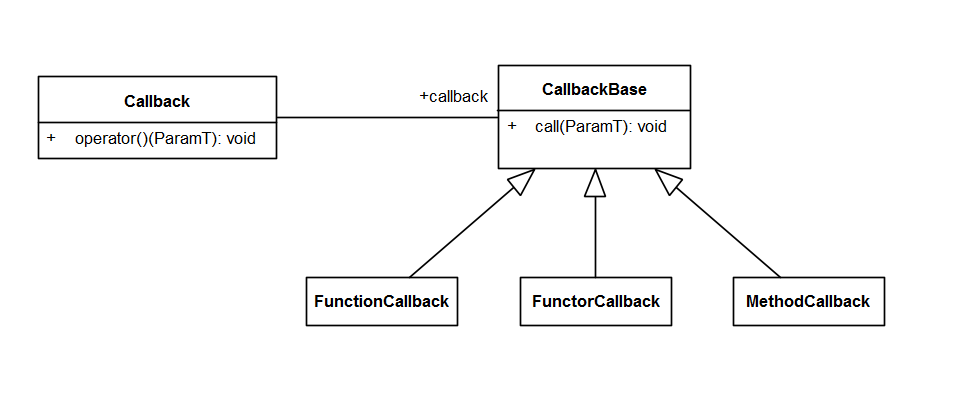
\includegraphics[width=.7\textwidth]{04_advanced/figures/callback_metamodel.png}
\end{center}

\paragraph*{\lstinline{CallbackBase}}

Fange mit der Klasse \lstinline{CallbackBase} an.
Damit man beim Aufrufen des Callbacks einen Parameter übergeben kann, füge \lstinline{call()} einen Parameter vom Typ \lstinline{ParamT} hinzu, wobei \lstinline{ParamT} ein Template-Parameter von \lstinline{CallbackBase} sein soll.
Der Klassenrumpf lautet also

\cpppInputListing{04_advanced/problems/listings/callbacks_base.hpp}

Falls ein Callback eigentlich mehrere Parameter erfordert, müssen diese entsprechend in ein Containerobjekt gepackt werden.
Generische Callback-Wrapper mit variabler Parameteranzahl sind zwar möglich, würden aber den Rahmen dieses Praktikums sprengen.

\hints{
    \item Du kannst diese und alle nachfolgenden Klassen in einem einzigen Header implementieren, weil die Klassen sehr kurz sind und außerdem semantisch stark zusammenhängen.
}

\subsection{Klasse \lstinline{FunctionCallback}}
Implementiere nun die erste Unterklasse \lstinline{template<typename ParamT> FunctionCallback}, die von \lstinline{CallbackBase<ParamT>} erbt.
\lstinline{FunctionCallback} soll einen entsprechenden Funktionszeiger als Attribut besitzen, der bei der Konstruktion initialisiert wird.
Ebenso soll \lstinline{call(ParamT t)} implementiert werden, in der der gespeicherte Funktionszeiger mit dem gegebenen Argument aufgerufen wird.

Teste deine Implementation.
Lasse \lstinline{hanoi()} einen Zeiger auf \lstinline{CallbackBase} erwarten, übergebe aber die Adresse eines \lstinline{FunctionCallback} Objektes.
Du kannst folgende Vorlage verwenden:

\cpppInputListing{04_advanced/problems/listings/callbacks_intpair.cpp}


\subsection{Klasse \lstinline{FunctorCallback}}
Implementiere nun die Unterklasse \lstinline{template<typename ParamT, typename ClassT> FunctorCallback}.
Zusätzlich zum Parameter-Typ muss hier auch der Typ der Funktor-Klasse angegeben werden.
Speichere das zu verwendende Funktor-Objekt als Referenz ab, um Kopien zu vermeiden.
Achte auch im Konstruktor darauf, dass keine Kopien des Funktors gemacht werden.
Teste deine Implementation!



\subsection{Klasse \lstinline{MethodCallback}}
Implementiere nun die letzte Unterklasse \lstinline{template<typename ParamT, typename ClassT> MethodCallback}.
Beachte, dass nun zwei Attribute nötig sind - ein Methodenzeiger und ein Zeiger auf das zu verwendende Objekt.
Teste deine Implementation.

\hints{
    \item Verwende beispielsweise folgende Signatur für den Konstruktor von \lstinline{MethodCallback}: \lstinline{MethodCallback(void(ClassT::*method)(ParamT), ClassT *object)}
    \item Gegeben einen Zeiger \lstinline{object} auf ein Objekt, einen Zeiger \lstinline{method} auf eines seiner Methoden und einen Parameter \lstinline{p} für die Methode, sieht ein Aufruf von \lstinline{method} wie folgt aus: \lstinline{(object->*method)(p);}
}

\subsection{Klasse \lstinline{Callback}}
Wir haben jetzt den Typ des Callbacks vollständig von seiner Verwendung entkoppelt.
Jedoch muss ein Callback-Objekt per Zeiger/Referenz übergeben werden, sodass das dir schon bekannte Problem der Zuständigkeit für die Zerstörung eines Objekts entsteht.
Außerdem muss man beim Erstellen eines Callbacks explizit den Typ der Unterklasse angeben.
Es wäre also sinnvoll, einen entsprechenden Wrapper zu schreiben, der sich um die Speicherverwaltung von Callbacks kümmert und bei der Konstruktion die passende Unterklasse selbst aussucht.

Schreibe eine Klasse \lstinline{template<typename ParamT> Callback}, die einen Smart Pointer auf ein \lstinline{CallbackBase}-Objekt als Attribut hat. Der Smart Pointer soll die Speicherverwaltung übernehmen. Überlade den \lstinline{operator()}, der den Aufruf einfach an das \lstinline{CallbackBase}-Objekt hinter dem Smart Pointer weiterleitet.

Implementiere nun für jede Callback-Art je einen Konstruktor, der eine Instanz der entsprechenden Unterklasse erzeugt und im Smart Pointer speichert.
Der erste Konstruktor soll also einen Funktionszeiger entgegennehmen und ein \lstinline{FunctionCallback} instantiieren.
Der zweite Konstruktor soll eine Referenz auf ein Funktor-Objekt erwarten und  \lstinline{FunctorCallback} instantiieren, und der dritte entsprechend ein \lstinline{MethodCallback}.
Beachte, dass die beiden letztgenannten Konstruktoren selbst Template-Methoden sind, da die \lstinline{Callback}-Klasse nur an den Parameter-Typ gekoppelt ist.

Teste deine Implementation in Zusammenhang mit der \lstinline{hanoi}-Funktion. Du kannst das \lstinline{Callback}-Objekt auch per Wert übergeben, da intern nur Zeiger kopiert werden.
